\documentclass[10pt,a4paper]{article}
\usepackage{graphicx} %LaTeX package to import graphics
\graphicspath{image/} %configuring the graphicx package,le immagini si trovano in image/
\usepackage{hyperref}
\usepackage{float}
\usepackage[utf8]{inputenc}
\usepackage[T1]{fontenc}
\usepackage{cite}
\usepackage{url}
\title{Ambliopia}
\author{Luca Frangiamore}

\date{2023}

\begin{document}
	
	\maketitle
	\tableofcontents{\tiny }
	
	
	\begin{abstract}
		Trattazione ambliopia mediante l'utilizzo di un applicativo mobile.
	\end{abstract} 
    \newpage
    \null
    \newpage
    
	 
	\section {Ambliopia}
	L'ambliopia, anche conosciuta come "occhio pigro" è una patologia che si manifesta nei prima anni dello sviluppo, età compresa tra 0-6 anni, il quale colpisce circa il 4\% della popolazione mondiale.
	La patologia riguarda la non corretta stimolazione dell'apparato visivo, in questo caso il cervello non riesce a ricreare l'immagine tridimensionale e quindi per evitare il fenomeno della visione doppia, anche detta \textbf{diplopia}, il cervello tenterà di sopprimere un immagine.
	Nella maggior parte dei casi, l'occhio è anatomicamente perfetto, \textbf{ambliopia funzionale}, in casi peggiori possiamo riscontrare \textbf{ambliopia organica} in cui vi è una deviazione delle vie ottiche.
	La seguente patologia si può manifestare con più probabilità in maniera asimmetrica, \textbf{monolaterale}, il quale colpisce un solo occhio, o più raramente possiamo trovare la forma \textbf{bilaterale}, il quale colpisce entrambi gli occhi.
	Normalmente l'ambliopia non peggiora durante la vita adulta in quanto oramai lo sviluppo alterato della vista si è oramai instaurato, l'età in cui l'ambliopia si stabilizzi in modo permanente va dagli 8 ai 15 anni.
	\subsection{Diagnosi}
	La diagnosi è un punto fondamentale per il trattamento dell'ambliopia, in quanto, una diagnosi tardiva può influire negativamente sulla corretta terapia, riducendo le possibilità di recupero.
	Il trattamento in genere viene personalizzata dal medico oculistico.
	\begin{itemize}
		\item Classica, in cui si cerca di stabilire l'acuità visiva e la visione binoculare del piccolo paziente. In caso di strabismo sarà necessaria anche una visita ortottica, la quale, è una branca dell'oftalmologia che si occupa della valutazione e riabilitazione di deficit muscolari e sensoriali.
		\item Pediatric Vision Scanner, Negli ultimi anni si sta sviluppando un nuovo metodo in grado di riconoscere l'ambliopia in età pediatrica con alta precisione.
		Come pubblicato nel articolo Validation of the Pediatric Vision Scanner in a normal preschool population, in cui si prende in esame Pediatric Vision Scanner(PVS), il quale scatta una foto ad entrambi gli occhi per poi andare a misurare errore di rifrazione e disallineamento.
			\begin{figure}[h]
				\centering
				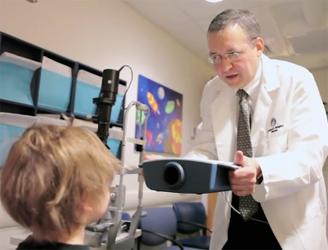
\includegraphics[width=0.7\linewidth]{image/pvs}
				\caption{Pediatric Vision Scanner\cite{PVS_image}}
				\label{fig:pvs}
	    	\end{figure}\\
        Il metodo in questione, descritto nell'articolo, ha permesso di identificare correttamente tutti e 6 i bambini con ambliopia e/o strabismo nel campione di 300 bambini, garantendo così una precisione del 100\%. Inoltre, il metodo potrebbe essere in grado di diagnosticare l'ambliopia già a partire dai 2 anni di età, suggerendo un potenziale miglioramento nella diagnosi precoce di questa patologia.
	
	\end{itemize}
   
	\subsection{Cause}
	In generale come detto prima, l'occhio pigro riguarda il progressivo trascuramento dei segnali di uno dei due occhi.
	Questo processo di sviluppo è causato da un non corretto sviluppo delle vie nervose degli occhi, le quali vengono stimolate in modo non bilanciate, ciò è dovuto magari dalla presenza di una condizione oculare presente in uno dei due occhio.
	Alcune condizioni che possono insorgere sono:
	\begin{itemize}
		\item Astigmatismo, visione è poco nitida e distorta in qualsivoglia direzione.
		\item Strabismo, deviazione degli assi visivi, impedisce il corretto coordinamento degli occhi. 
		\item Cataratta, opacizzazione parziale o totale del cristallino,  causa offuscamento e difficoltà nel mettere a fuoco le immagini.
		\item Ptosi palpebrale, una o entrambi le palpebre sono superiori sono abbassate più del normale.
	\end{itemize}
	Come detto prima, se il cervello non riesce a combinare le immagini proveniente dai due occhi, esso può decidere di trascurare un dei due segnali, prediligendo l'occhio ottimale, sviluppando quindi l'ambliopia.
	\subsection{Sintomi}
	Vi sono alcuni casi, in cui il paziente probabilmente giovane, non si accorge della patologia, questo può ritardare o eliminare i trattamenti attui a ridurre o eliminare il problema.
	Tra i problemi più comuni possiamo citare:	   
	\begin{itemize}
		\item Difficoltà dei visione in un occhio.
		\item Movimenti involontari dell'occhio.
		\item Sensibilità al movimento compromessa.
		\item Scarsa percezione della profondità in quanto viene meno la coordinazione tra i due occhi.
	\end{itemize} 
\newpage   
	\subsection{Trattamenti}
	Subito dopo aver riconosciuto il disturbo bisogna procedere con la corretta terapia.Come prima cosa, bisogna corregge il difetto che ha portato l'inibizione dell'occhio pigro, successivamente si procede con la terapia occlusiva, la quale permette di stimolare l'occhio pigro.
	\begin{itemize}
		\item Patching, La terapia consiste nel coprire l'occhio dominante, da applicare per un perioda di tempo variabile.
		Il trattamento è efficacie, ma il recupero della vista impiega diversi mesi.       	   
			\begin{figure}[!h]
				\centering
				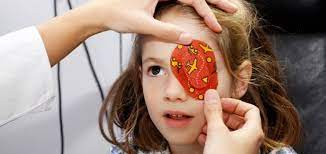
\includegraphics[width=0.8\linewidth]{image/patching}
				\caption{Trattamento con Patching.Fonte\cite{Patching_image}}
				\label{fig:patching}
			\end{figure}	
	
		\item Lenti opacizzazione, usate per limitare la visione dell'occhio sano e stimolare l'occhio pigro a lavorare di più. Un articolo che ha esaminato gli effetti delle lenti di Bangerter sulla funzione binoculare in pazienti con ambliopia è The effect of Bangerter filters on binocular function in observers with amblyopia.
			\begin{figure}[h]
				\centering
				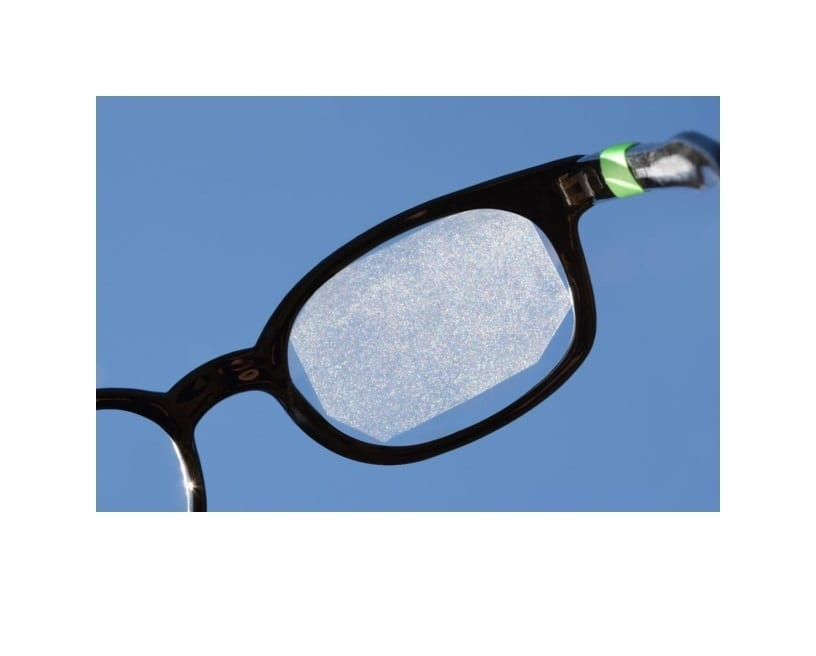
\includegraphics[width=0.7\linewidth]{image/penalizzazione ottica}
				\caption{Trattamento con lente di bangerter.
					Fonte\cite{Bangerter_image}}
				\label{fig:penalizzazione-ottica}
			\end{figure}
		\item Lenti a griglia,usate per impedire all'occhio sano di prendere il sopravvento nella visione, creando una situazione in cui l'occhio ambliope deve fare un maggiore sforzo per vedere e sviluppare la sua capacità visiva
		\lenti grigliate.
    	\newpage
		\item Collirio, permette di offuscare la vista dell'occhio dominante, in modo da poter stimolare il l'occhio più debole
		
		\item Luminopia, è un software approvato da  \textbf{Food and Drug Administration(FDA)} come annunciato dal CEO Scott Xiao, che permette ai pazienti di poter usufruire di 700 ore di serie o film, adattati tramite AI. Questo sistema permette di rendere il trattamento dell'ambliopia piacevole e quindi sopportabile nel lungo periodo.
		I pazienti usufruiscono di questi contenuti mediante il vr, in modo da poter visionare i contenuti scelti.
			\begin{figure}[h]
				\centering
				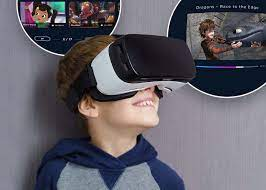
\includegraphics[width=0.7\linewidth]{image/luminopia}
				\caption{Trattamento innovativo con Luminopia.Fonte\cite{Lumiopia_image}}
				\label{fig:luminopia}
			\end{figure}
	    \item Esiste poi un altro tipo di tecnologia, I-BiT Plus\cite{I-Bit}, il quale permette al paziente di intrattenersi mediante giochi interattivi o video.
	    \begin{figure}[h]
	    	\centering
	    	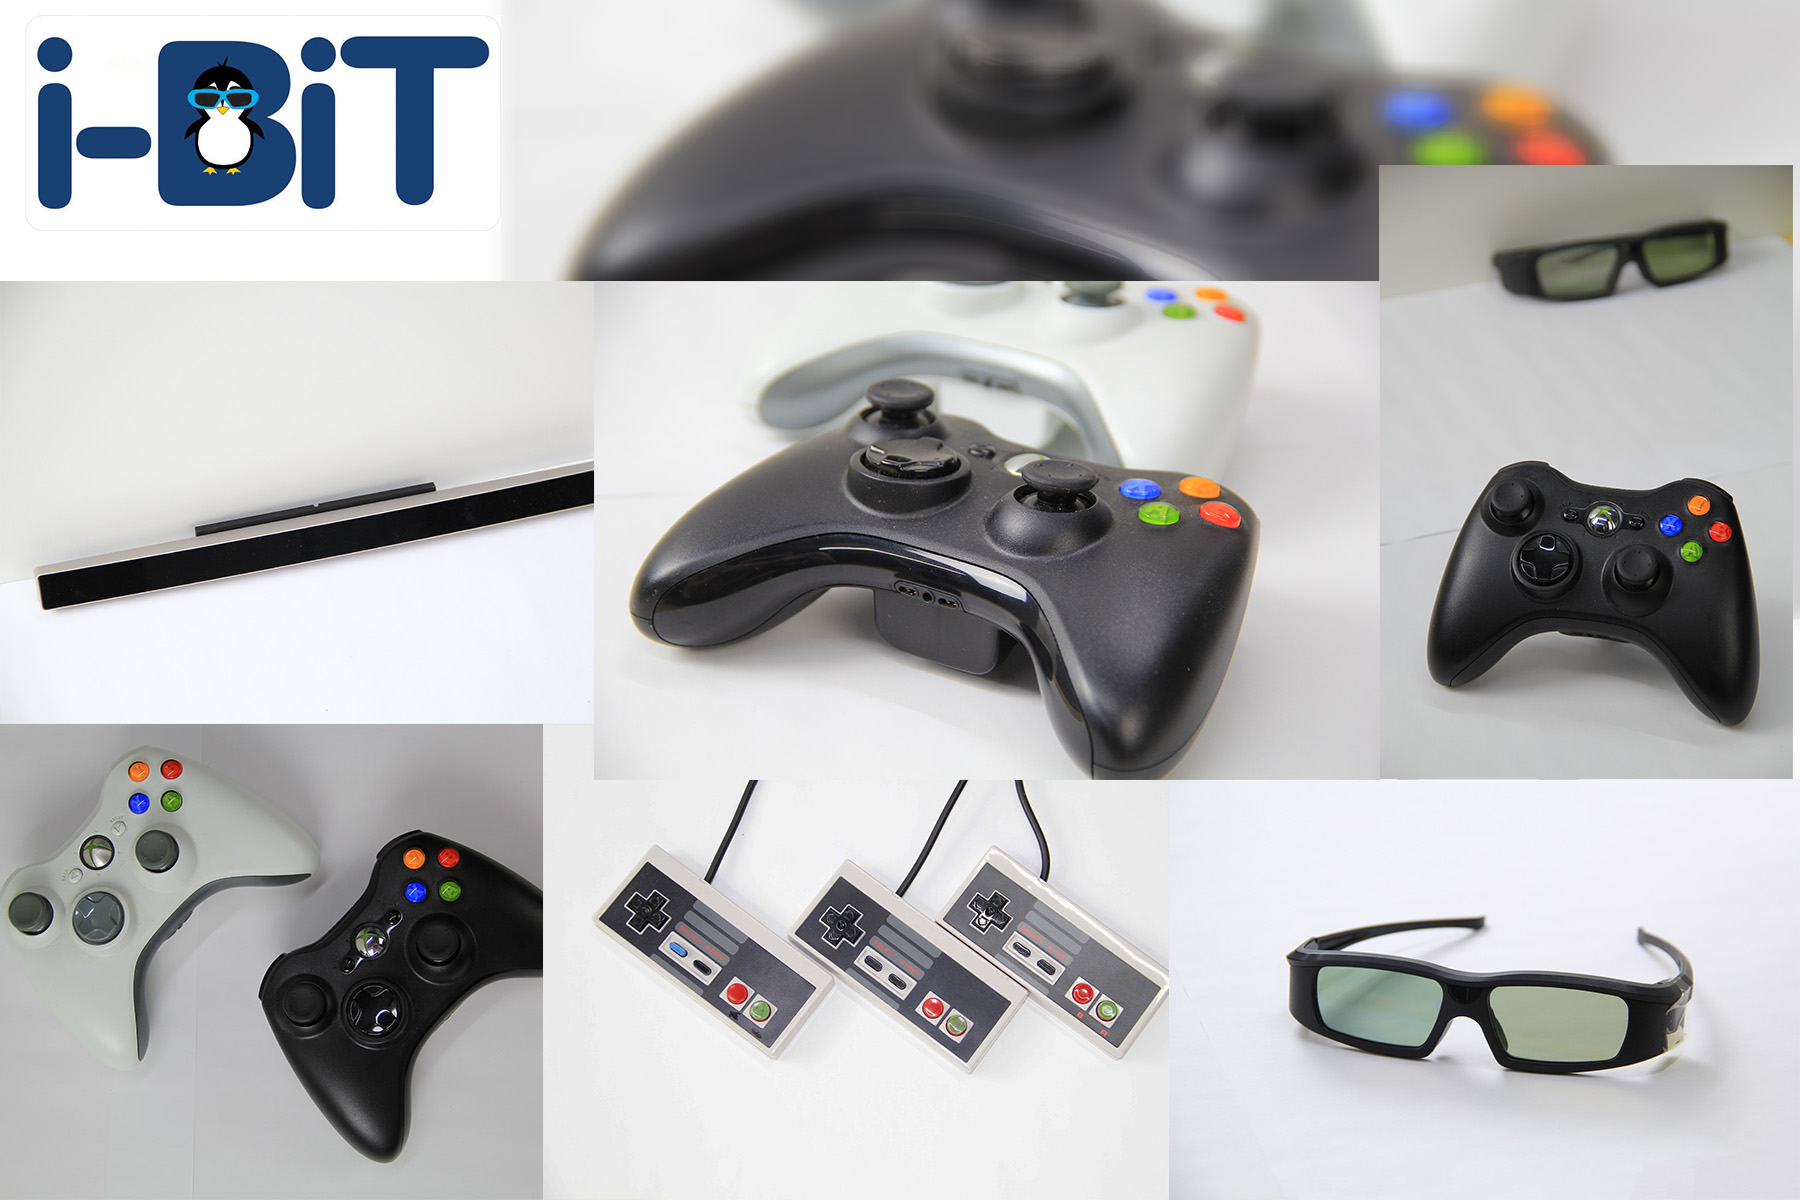
\includegraphics[width=0.7\linewidth]{image/I_bit}
	    	\caption{I bit.Fonte\cite{I-Bit}}
	    	\label{fig:I_bit}
	    \end{figure}
	    Il suo funzionamento si baso sul mostrare la parte più "interessante" del gioco o DVD, come ostacoli o obiettivi, mentre nell'occhio pigro vengono mostrati oggetti di contorno, come i paesaggi.
	    Per assicurare che il paziente continui a guardare le immagini in un posizione ottimale il sistema si serve di un Eye tracker, in modo da garantire il coretto posizionamento dell'immagine.
	    
    \end{itemize}
\newpage
\null
\newpage

	\section{3D4Amb}
	Il progetto è nato con l'intenzione di, creare uno strumento utile ed economico per il trattamento, misurazione dell'occhio pigro basato sul 3D.
	
	\subsection{Funzionamento e strumenti}
	Il funzionamento di base è sempre lo stesso, si va a mostrare al paziente due immagini diverse ma correlate tra loro, pre-elaborate tramite il software 3D4Amb.
	3D4Amb utilizza diversi supporti tecnologici, il quale ci permette di realizzare delle applicazione video ludiche basate sulla differenziazione delle immagini,come detto sopra, il tutto relativamente a basso costo.
	Per poter utilizzare 3D4Amb bisogna garantire lo sdoppiamento delle immagine per i due occhi, le quali dovranno essere mostrate ai due occhi, per garantire il coretto sdoppiamento, si sono sperimentate diverse strade.
	\subsubsection{Cardboard}\label{chap:cardboard}
    Il funzionamento del Google Cardboard,fig:\ref{fig:cardboard}, si basa sulla creazione di un effetto stereoscopico\cite{Stereoscopio}, utilizzando uno smartphone, che viene inserito all'interno del dispositivo
	Il cardboard utilizza due lenti che permettono di ingrandire l'immagine fino ad riempire il campo visivo\cite{Funzionamento_cardboard}.
	\begin{figure}[H]
		\centering
		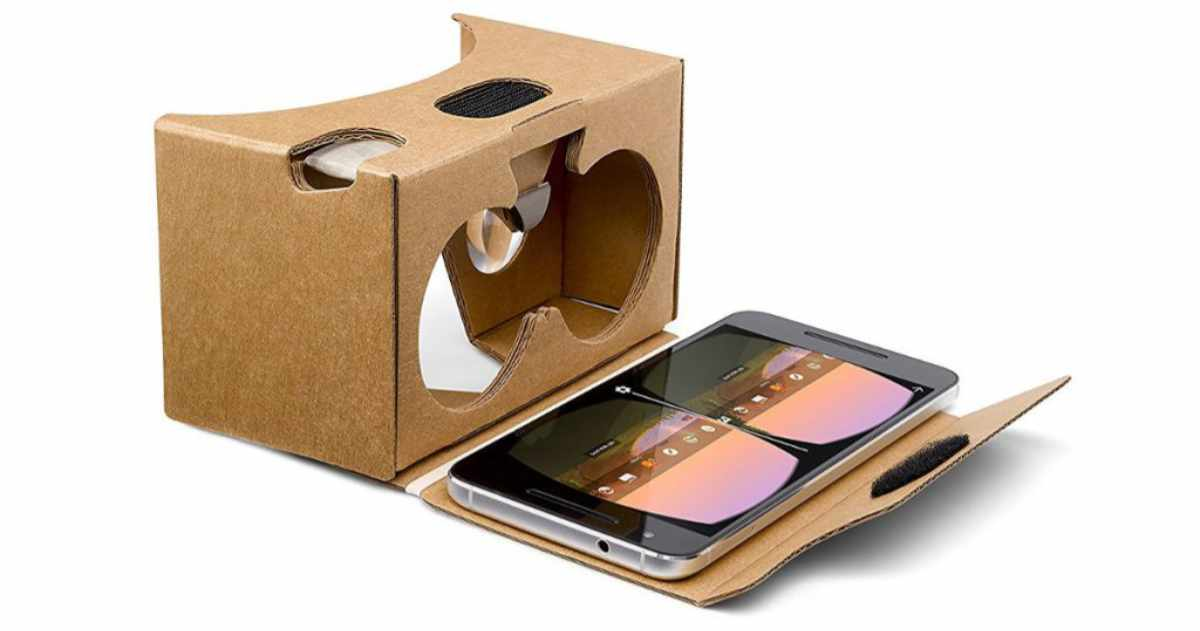
\includegraphics[width=0.8\linewidth]{image/cardboard}
		\caption{Cardboard di cartone.Fonte\cite{Cardboard_image}}
		\label{fig:cardboard}
	\end{figure}
	Questo dispositivo ci permette di poter usufruire della tecnologia 3D con un costo relativamente basso che si aggira sui 10\$, esso ci permette di mostrare e/o alterare alcuni elementi i una delle due lenti, in cui si trova l'occhio sano. 
	\begin{figure}[H]
		\centering
		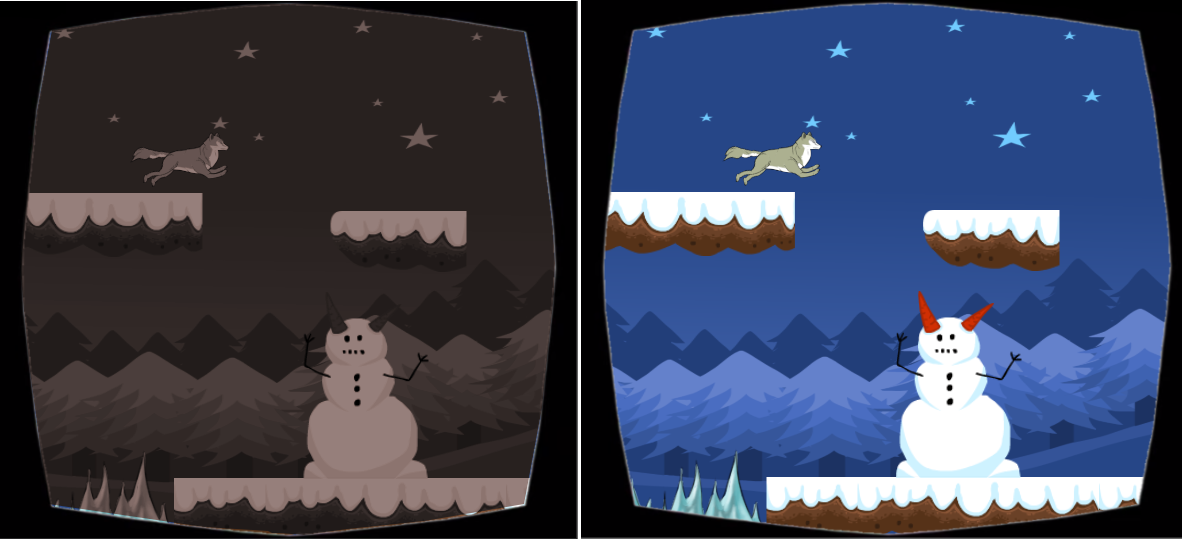
\includegraphics[width=0.8\linewidth]{image/3D4Amb_1}
		\caption{Differenziazione colori.
			Fonte\cite{3d4amb_image}}
		\label{fig:cardboard-3D4Amb_colori}
	\end{figure}
   
    Come mostrato nella fig:\ref{fig:cardboard-3D4Amb_colori}, le immagini mostrate differisco per il colore, vi sono casi in cui si può andare ad omettere un elemento della scena fig:\ref{fig:cardboard-3D4Amb_elementi}
    	\begin{figure}[H]
    	\centering
    	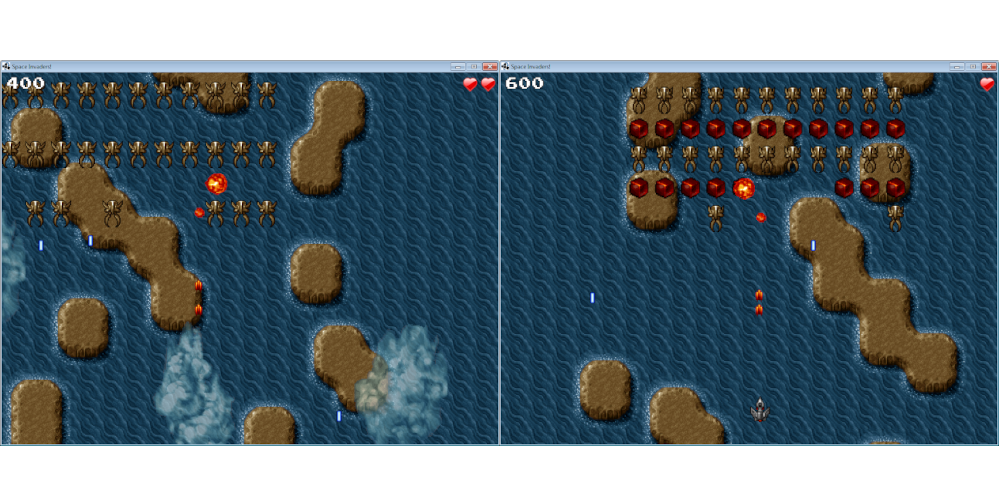
\includegraphics[width=0.8\linewidth]{image/3D4Amb_2}
    	\caption{Differenziazione elementi su schermo.Fonte\cite{3d4amb_image}}
    	\label{fig:cardboard-3D4Amb_elementi}
    \end{figure}
    Oltre alle caratteristiche menzionate prima bisogna specificare che il cardboard non nè altro che uno strumento che mi permette di dividere le immagini emesse da telefono, che risiede al suo interno, questo implicitamente significa che potremmo sfruttare tutte le possibilità che il telefono ci offre.

	\subsubsection{Occhiali Anaglifici}\label{chap:occhiali_anaglifici}

	Gli occhiale fig:\ref{fig:occhiali_anaglifici}, sono provvisti da due lenti dette anche  filtri in \textbf{gelatina rossa e ciano}, i quali vengono usati per poter osservare un immagine composta da due immagini. 
	\begin{figure}[H]
		\centering
		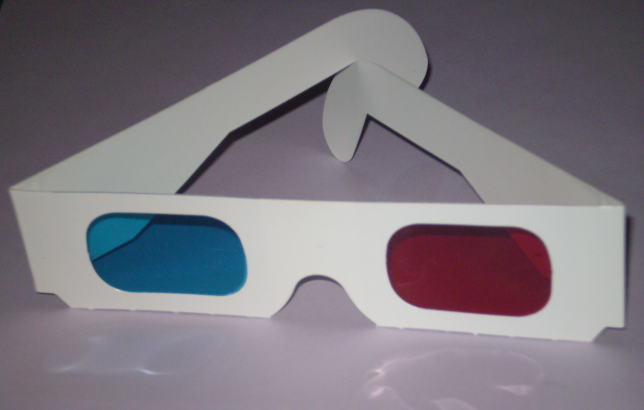
\includegraphics[width=0.7\linewidth]{image/occhiali_anaglifici}
		\caption{occhiali anaglifici.Fonte\cite{Anaglifo_image}}
		\label{fig:occhiali_anaglifici}
	\end{figure}
	Le immagini sono distanti tra loro(generalmente 5,7 cm), con colori complementari fig:\ref{fig:anaglifo}, gli occhiali vengo usati per poter osservare solo l'immagine cromatica complementare, questo permette di ricreare l'effetto tridimensionale.
	 \begin{figure}[H]
	 	\centering
	 	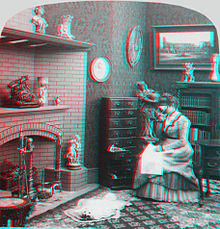
\includegraphics[width=0.7\linewidth]{image/anaglifo}
	 	\caption{Anaglifo.Fonte\cite{Anaglifo_image}}
	 	\label{fig:anaglifo}
	 \end{figure}
 \newpage
	\subsubsection{Active shutter 3D system}
	Questo tipi di tecnologia ci permette di mostrare delle immagine in rapida successione, un volta nel occhio di destra, una quello di sinistra, questa operazione viene fatta con alta frequenza, creando quindi la sensazione di visione tridimensionale, a differenza del cardboard cap:\ref{chap:cardboard}, in cui le immagini sono mostrate contemporaneamente.
		\begin{figure}[H]
		\centering
		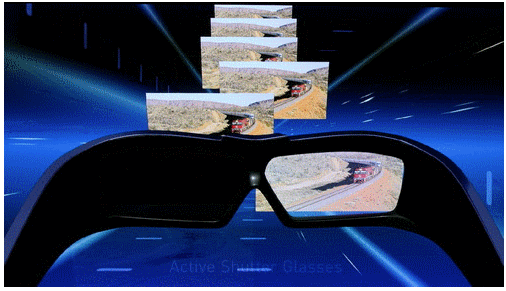
\includegraphics[width=0.8\linewidth]{image/active-shutter-3d-technology}
		\caption{Differenziazione elementi su schermo.\newline
			Fonte\cite{active-shutter-3d_image}}
		\label{fig:occhiali active-shutter-3d-technology}
	\end{figure}

	\subsection{Obiettivi}
	Utilizzando la tecnologia 3D è possibile trattare l'ambliopia, attraverso un approccio ludico, permettendo quindi di intrattenere maggiormente il paziente, spesso in età giovanile, aumentando quindi la probabilità di successo.
	I punti in cui 3D4Amb si focalizza sono:
	\begin{itemize}
		\item Basso costoso, il sistema si basa su tecnologie a basso costo.
		\item Facile da usare, non richiede nessun particolare capacità, permettendo anche ai pazienti più piccoli di poter usufruire del sistema senza l'assistenza dei genitori.
		\item Uso domestico, il sistema può essere utilizzato nel ambiente domestico, evitando quindi le visite frequenti all'ospedale
		\item Facilmente estendibile, 3D4Amb permette di usare le librerie software, agevolando  quindi l'estensione del sistema, aggiungendo nuove applicazione o funzioni.
	\end{itemize}
    \newpage
    \null
    \newpage

    \section{Progetto}
    L'obiettivo di questa tesi è quello di andare a trattare l'ambliopia mediante uno strumento che sia in grado di intrattenere maggiormente il paziente.  
    Il videogioco implementato, utilizza uno strumento per sdoppiare le immagini, il cardboard, cap:\ref{chap:cardboard}.
    Come genere ho deciso di implementare un FPS(First Person Shooter), in modo tale da costringere il pazienze ad osservare e/o girare l'ambiente circostante, sin nei minimi particolari, cosa che era più difficile da realizzare mediante altri generi, il tutto è stato reso più immersivo mediante l'utilizzo come detto in precedenza del cardboard.
    Oltre al genere FPS, ho anche deciso di utilizzare dei toni fanciulleschi, in modo da poter alleggerire il più possibile la terapia.
    L'intento ludico del gioco risiede nel fattore di progressione tra i vari livelli.
    Per l'interazione con l'ambiente ho deciso di utilizzare un gamepad, il quale mi permetti di avere un buon numero di tasti, che si traduce in maggiori interazioni.
     \begin{figure}[H]
    	\centering
    	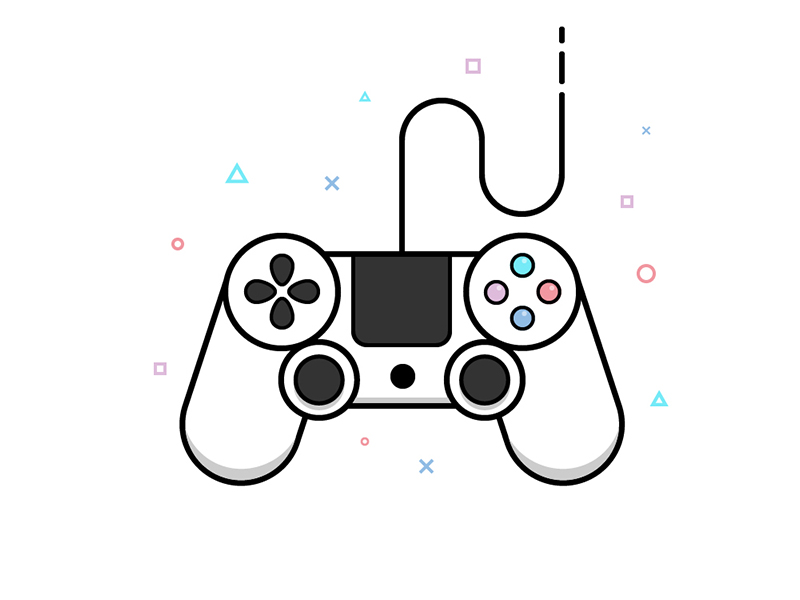
\includegraphics[width=0.8\linewidth]{image/gamepad}
    	\caption{Layout gamepad utilizzato.Fonte\cite{controller_image}}
    	\label{fig:gamepad}
    \end{figure}
  
    \subsection{Tecnologie utilizzate}
    Nel era moderna, le tecnologie disponibili sono diverse, per la realizzazione del progetto mi sono avvalso delle seguenti tecnologie:
    \begin{itemize}
    	\item:Cardboard, 
    	\item:Unity 3D, motore di gioco
    	\item:Visual Code, editor di codice sorgente
    	\item:Blender, creazione di elementi 3D
    \end{itemize}
  \subsubsection{Cardboard, motivi della scelta}\label{chap:cardboard_motivi}
    La motivazione che mi ha portato a scegliere il cardboard e non gli occhiali anaglifici, cap:\ref{chap:occhiali_anaglifici}, risiedono principalmente nella sua versatilità, visto che mi permette di poter realizzare un applicazione con limitati limiti tecnici e con un budget ridotto, fatto cruciale, visto che si parla principalmente di un'applicazione idealmente indirizzata per pazienti giovanissimi, i quali potranno usufruire dei sui benefici comodamente da casa.
    Una delle tecnologie che più mi è tornata utile del cardboard e quindi dello smartphone, è il giroscopio, il quale mi a permesso di realizzare un immersione maggiore.
    \subsubsection{Unity 3D}\label{unity3D}
    Unity 3D è un motore di gioco sviluppato dalla Unity
    Technologies, il quale permette di realizzare dei videogiochi tridimensionali e bidimensionali, la sua comunity e le varie guide messe a disposizione da unity permettono di cimentarsi in questo progetto superando il plateau d'apprendimento.
    Si tratta di uno strumento che permette di alleggerire il processo di produzione attraverso l'utilizzo di un interfaccia grafica ben organizzata, vi sono 4 schermate principali:
    \begin{itemize}
    	\item Scene, Permette di spostare e/o modificare gli oggetti nella scena.
    	\item Simulator, Permette di eseguire l'applicativo.
    	\item Inspector, Il quale mette a disposizione delle impostazione di modifica.
    	\item Hierarchy, Mostra i vari elementi nella scena.
    \end{itemize}
    \begin{figure}[H]
    	\centering
    	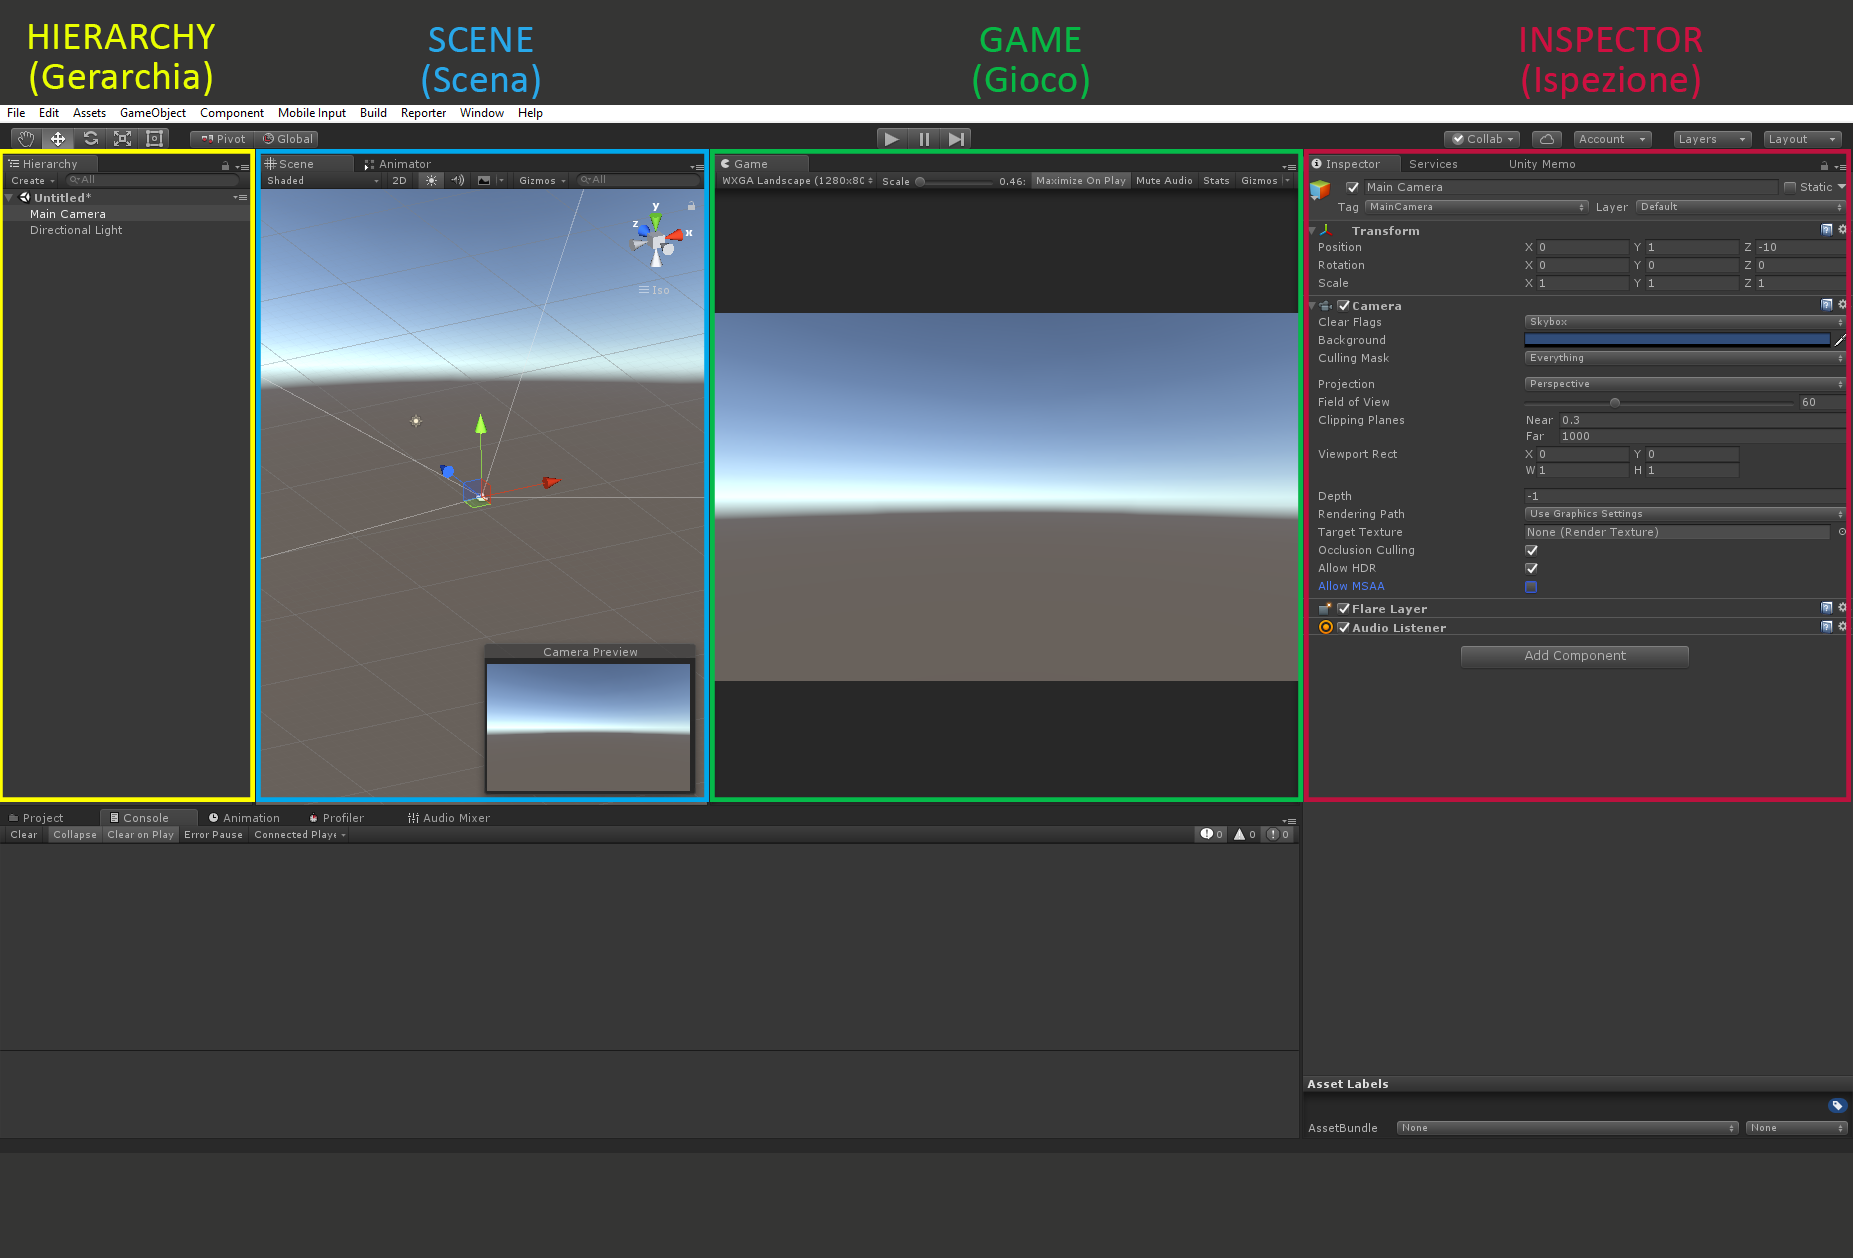
\includegraphics[width=0.8\linewidth]{image/unity}
    	\caption{Schermate unity}
    	\label{fig:unity}
    \end{figure}
    Questo motore di gioco ci permette di poter realizzare i propri prodotti indipendentemente dalla piattaforma per poi andare a costruire la versione apposita, senza dovere effettuare nessuna modifica.
    Una funzione molto importante per questo progetto è stata la simulazione su dispositivo android, il quale mi ha permesso di poter provare l'applicativo direttamente sul mio telefono con il cardboard, cap:\ref{chap:cardboard}, e al contempo interagire e/o modificare la scena senza avere la necessita di dover buildare il tutto sul telefono.
    \textbf{L'Asset Store}è una delle caratteristiche che io ho trovato fondamentale è la presenza del Asset Store, ovvero unity3D, mette a disposizione una serie di oggetti, anche pubblicati dal utente, che permettono di tralasciare alcuni aspetti in modo da potersi concentrare su altro.
    Il materiale presente sull'Asset Store va dal semplice oggetto 3D,script a veri e propri pacchetti.
    Al interno dell'Asset Store è possibile quindi trovare tutti gli elementi utili per poter sviluppare un gioco da zero, volendo anche gratuitamente.
    \subsubsection{Visual code}
    Visual code è un editor di codice usato in correlazione con unity 3D per la realizzazione degli script di gioco.
    Visual Studio Code è un editor di codice sorgente sviluppato da Microsoft che ha guadagnato rapidamente popolarità tra gli sviluppatori. È gratuito, multipiattaforma e altamente personalizzabile grazie all'ampia gamma di estensioni disponibili attraverso il marketplace integrato.
    Una delle caratteristiche distintive di Visual Studio Code è la sua interfaccia utente pulita e intuitiva. L'editor utilizza una combinazione di barre degli strumenti, pannelli laterali e schede per fornire un accesso rapido alle funzionalità chiave.
    Un'altra caratteristica importante di Visual Studio Code è la sua capacità di supportare molteplici linguaggi di programmazione.
    \begin{figure}[H]
    	\centering
    	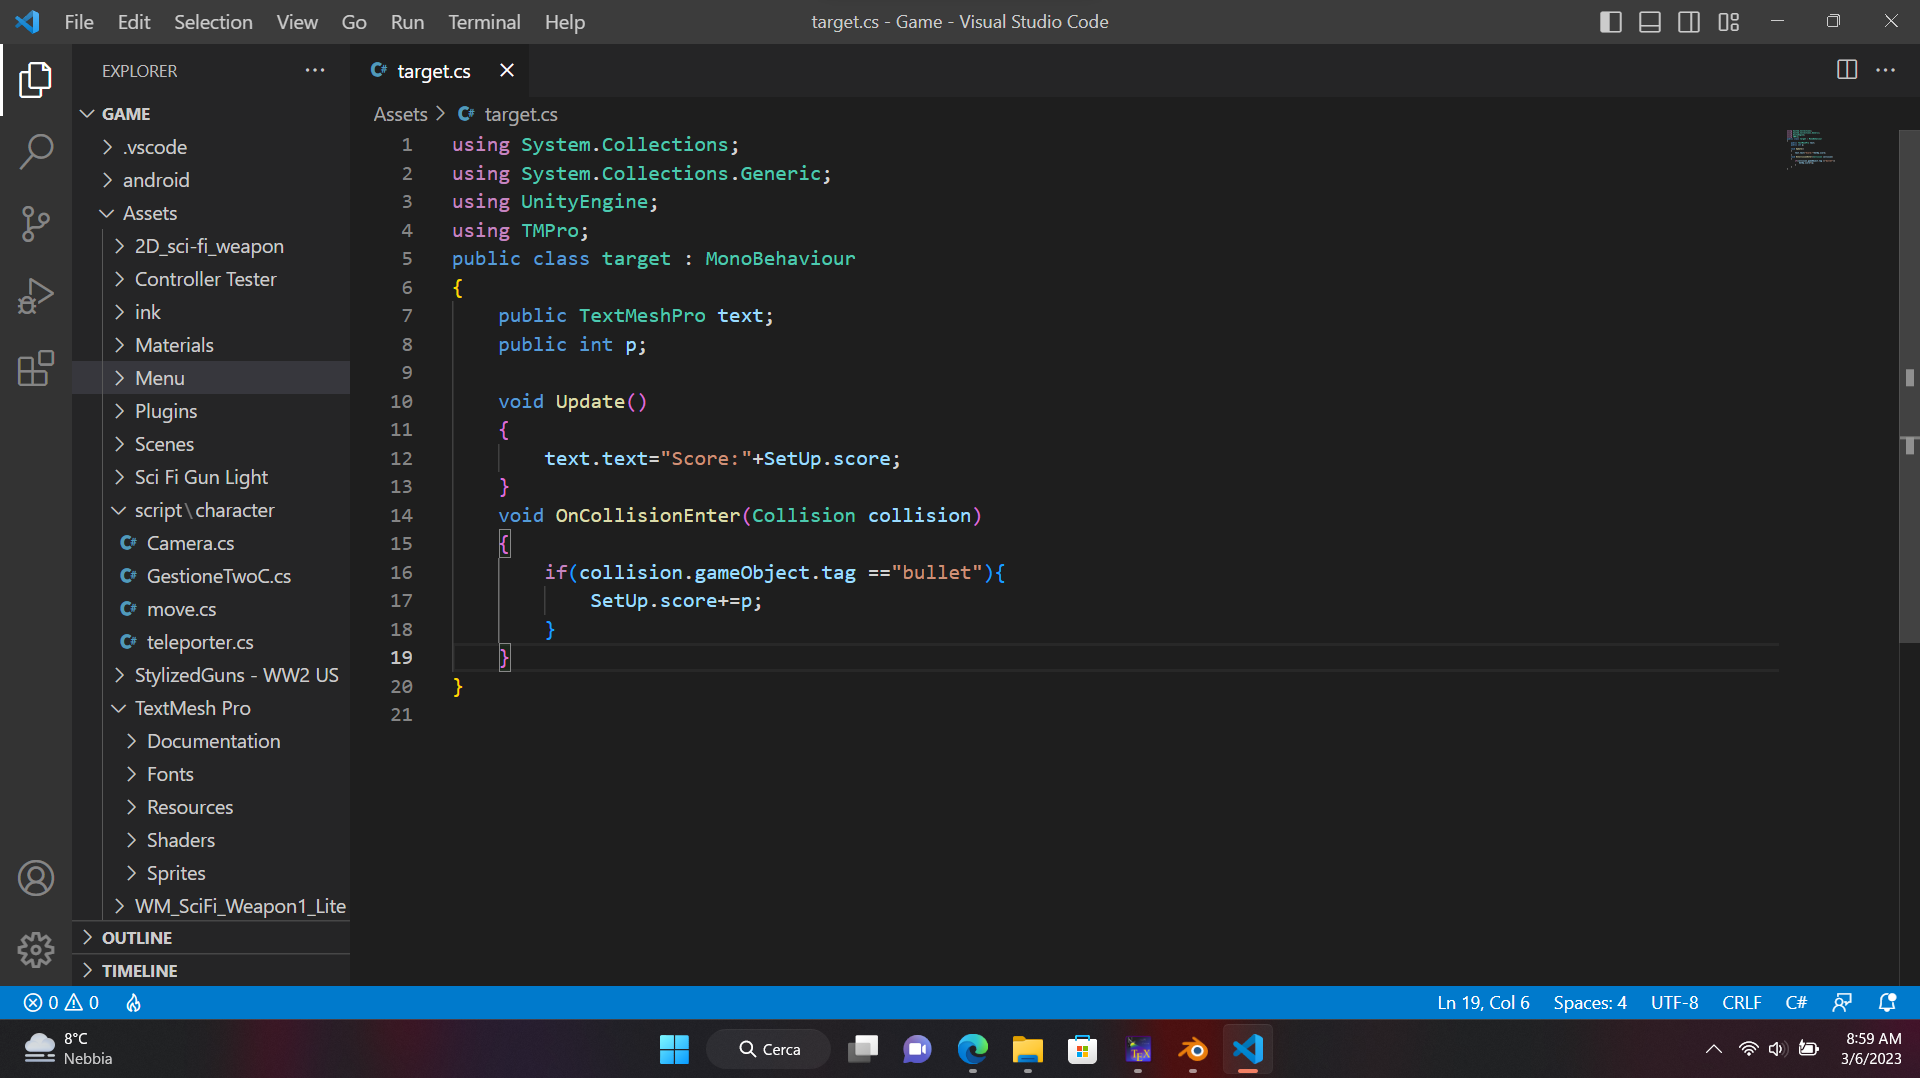
\includegraphics[width=0.8\linewidth]{image/visual_code}
    	\caption{Esempio di script realizzato con visual code}
    	\label{fig:visual_code}
    \end{figure}
    Le estensioni utilizzate in questo progetto riguardano principalmente l'interazione con unity 3D:
    \begin{itemize}
    	\item Unity code snippets, usato per introdurre l'auto completamento di porzioni di codice standard.
    	\item Unity tools, installato per poter consultare la documentazione in modo facile e dinamico. 
    \end{itemize}
    \subsection{Struttura}
    La struttura dell'applicativo è molto lineare, bisogna raccogliere dei punti mediante l'interazione con determinati oggetti sparsi per la mappa, denominati \textit{target} , una volta fatto ciò, si procede al livello successivo.
    Ogni livello ha una mappa e una diverso livello di \textit{trasparenza}, argomento che verrà trattato maggiormente nei capitoli successivi.
    La struttura dei livelli è molto lineare, in diversi punti della mappa vi sono diversi obiettivi a cui bisogna sparare, ogni target permette al paziente di ottenere dei punti, dopo aver ottenuto un determinato punteggio si aprirà un portale che condurrà al livello successivo.
    Come detto in precedenza ciò che cambia non è solo la mappa, ma anche il livello di trasparenza, ovvero al interno dell'ambiente vi sono degli oggetti denominati \textit{OcchioMalato}, i quali verranno mostrati trasparenti all'occhio sano e solidi a quello pigro.
    \begin{figure}[H]
    	\centering
    	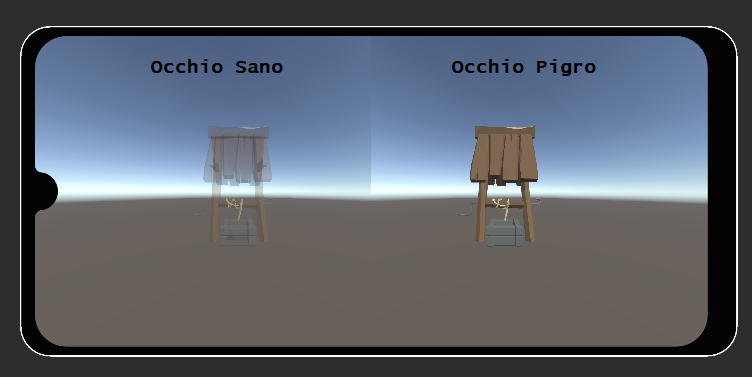
\includegraphics[width=0.8\linewidth]{image/Pr_trasparenza}
    	\caption{Esempio di trasparenza mediante un oggetto di gioco}
    	\label{fig:pozzo}
    \end{figure}
    Nella figura \ref{fig:pozzo}, possiamo notare come hai due occhi venga mostrato lo stesso oggetto ma con diversa trasparenza, in questo modo sollecitiamo l'occhio afflitto da ambliopia, lasciando anche una traccia all'occhio.
    Il livello di trasparenza varia ad ogni fase di gioco, esso aumenterà(gli oggetti diventeranno più trasparenti) man mano che si avanzerà di livello, in modo da poter stimolare efficacemente l'occhio con il passare dei livelli.
    \subsubsection{Target}
    Oggetti fondamentali, utilizzati per rendere l'esperienza più video ludica, dando al paziente un obiettivo da portare a termine, con difficoltà crescente, in modo da rendere il tutto più intrattenente per il lungo periodo.
    \begin{figure}[H]
	  	\centering
	  	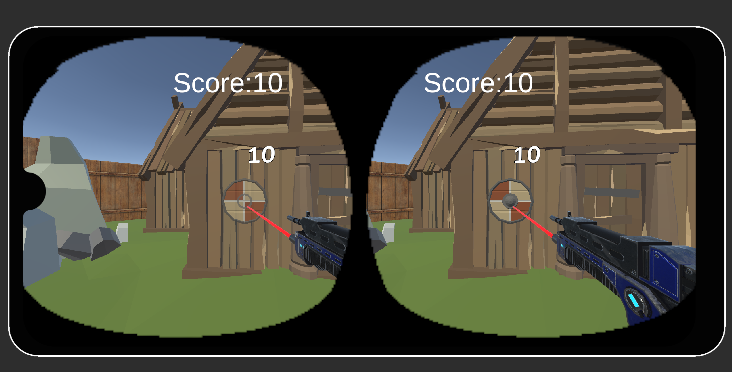
\includegraphics[width=0.7\linewidth]{image/target_score}
	  	\caption{Target con punteggio}
	  	\label{fig:target_score}
    \end{figure}
    
    I target sono principalmente degli scudi medievali,fig:\ref{fig:target_score}, i quali sono sparsi all'interno dei vari livelli di gioco.
    
    Essi si possono trovare in diverse forme:
    \begin{itemize}
       \item Scudo Classico, mostrato in fig:\ref{fig:target_score}, in questo caso la difficoltà risiede nel loro posizionamento.
       \item Scudo in Movimento, mostrato in fig:\ref{fig:target_movimento}, caratterizzato dal fatto che l'oggetto è in movimento, costringendo quindi il paziente a seguire l'oggetto con  lo sguardo, cosa che diventerà più difficile con il progredire dei livelli, sia per la velocità, che per il fatto trasparenza.
      \end{itemize}
  \begin{figure}[H]
  	\centering
  	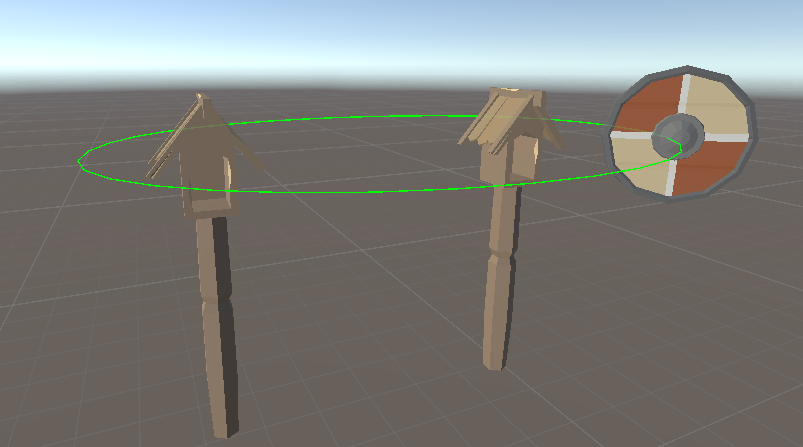
\includegraphics[width=0.7\linewidth]{image/target_movimento}
  	\caption{Target in movimento}
  	\label{fig:target_movimento}
  \end{figure}
    \subsection{Implementazione}
    Per l'implementazione ho deciso di utilizzare Unity 3D come motore di gioco, cap:\ref{unity3D}, per l'interazione ho optato per il semplice gamepad in modo da poter interagire efficacemente con il mondo di gioco.Come si può evincere dal genere scelto, ho optato per una visuale in prima persona, in modo da restituire un effetto più immersivo, concetto che verrà ripreso più avanti.
    Il flusso di lavoro è stato diviso principalmente in due parti:
    \begin{enumerate}
        \item Fase di prototipazione, in questa fase sono andato a definire i requisiti di progetto e la loro fattibilità, dopo aver fatto ciò, sono andato a sviluppare le componenti principali, il tutto è stato fatto all'interno di un ambiente di testing.
        \begin{figure}[H]
        	\centering
        	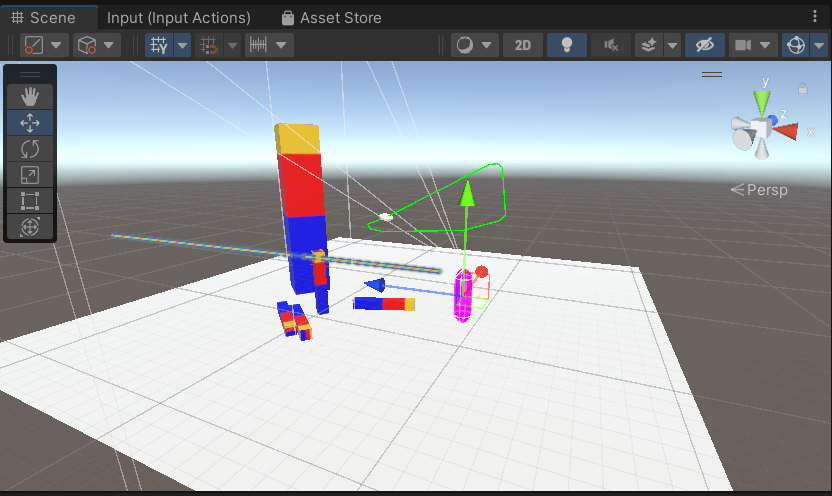
\includegraphics[width=0.8\linewidth]{image/protot}
        	\caption{Scena prototipale}
        	\label{fig:protot}
        \end{figure}
        \item Fase di sviluppo, dopo aver definito i vari requisiti ed aver sviluppato le componenti fondamentali mi sono cimentato nella creazione effettiva dei vari livelli, in cui sono andato ad utilizzare le componenti sviluppate nella fase prototipale.
    \end{enumerate}
    \subsubsection{Fase di prototipazione}
     Come detto in precedenza, in questa fase sono andato a definire le componenti principale del progetto:
     \begin{itemize}
     	\item Visuale, in cui mi sono occupato gestire due visualizzazione differenti.
     	\item Mappatura dei tasti, in cui ho definito i tasti utilizzati e le azioni a esse collegate.
     	\item Menu, in cui ho implementato i menù di scelta con le relative finestre.
     \end{itemize}
  
     \textbf{Per la visuale}, la preoccupazione più grande è stata ideare un sistema che permettesse di splittare le immagini dirette nei rispettivi occhio, per fare ciò ho usato due telecamere.
     Le due telecamere sono state poste alla distanza interpupillare media, 62mm\cite{Distanza_occhi}.
     Come accennato prima, le telecamere mostrano oggetti diversi, ovvero, oltre alla loro distanza, utile per ricreare l'effetto tridimensionale, mi sono anche preoccupato di trovare uno stratagemma che mi permettesse di mostrare lo stesso oggetto in maniera differente, effetto trasparenza.
     \textbf{L'effetto trasparenza} in questo caso è stato ricreato andando a sfruttare la possibilità di unity3D di poter duplicare gli oggetto, attraverso il metodo \textit{Instantiate} identificati con il tag "OcchioMalato", per poi andare ad utilizzare lo stesso materiale ma con un effetto di trasparenza.
     E per concludere vado a mostrare la copia(trasparente) al occhio sano, mentre l'originare(non trasparente) all'occhio pigro.
     Utilizzo questo meccanismo in ogni livello, andando a variare la gravita della trasparenza.\\\\
     \textbf{Per la mappatura} mi sono preoccupato di associare ogni tasto ad una specifica funzione, in modo da ricreare, una facile ergonomia, in modo tale da poter riconoscere i tasti principali senza l'utilizzo vederli, in quanto durante l'esperienza è richiesto l'uso del cardboard.
     Di seguito, fig:\ref{fig:gamepad_tasti}, riporto il layout dei tasti con le funzioni associate.
     Ho raggruppato la presentazione in 2 macro gruppi:Azioni personaggio e Navigazione menu.
     \begin{figure}[H]
     	\centering
     	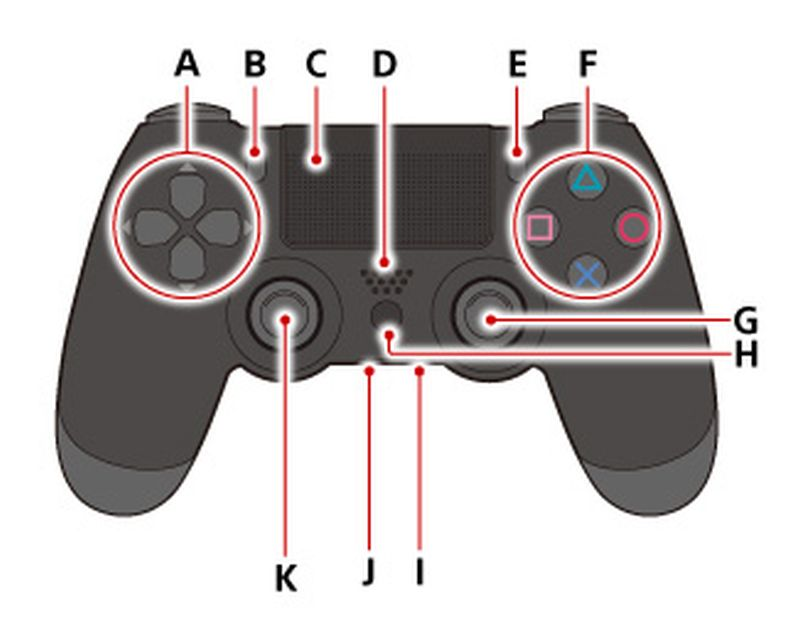
\includegraphics[width=0.8\linewidth]{image/gamepad_tasti}
     	\caption{Mappatura tasti}
     	\label{fig:gamepad_tasti}
     \end{figure}
      Per il macro gruppo, azioni del personaggio, vado ad elencare tutte le possibilità date al paziente, per navigare e interagire con i vari livelli dati a disposizione.
     \begin{itemize}
     	\item Movimento tridimensionale.\textit{Stick G}
     	\item Teletrasporto.\textit{Stick K}
     	\item Sparo.\textit{Dorsale RT}
     	\item Accucciarsi,Abbassarsi.\textit{Tasto stick G}
     	\item Voltarsi.\textit{RB+Stick G}
     	\item Sporgesi.\textit{D Pad:A Tasti orizzontali}
     	\item Riposizionamento telecamera.\textit{Tasto triangolo}
     \end{itemize}
     Per il macro gruppo, navigazione dei menu, vado ad elencare l'insieme dei tasti attui ad utilizzare correttamente il menu.
      \begin{itemize}
     	\item Apertura:\textit{Tasto E}
     	\item Chiusura:\textit{B}
     	\item Pagina precedente:\textit{Tasto E}
     	\item Navigazione opzioni.\textit{D Pad Tasti verticali}
     	\item Selezionare:\textit{Tasto quadrato}
     \end{itemize}
     Come si può evincere, vi sono tasti non assegnati, questo implica la possibilità di espandere il gioco mediante l'implementazione non solo di nuovi livelli ma anche di nuove funzioni.\\\\
     Nella creazione dei menu, mi sono concentrato a cercare un sistema che rispettasse il concetto di stereogramma\cite{Stereogramma}. Ho notato che i classici strumenti di Unity per la creazione dei menu non permettevano di rispettare il principio fondamentale dell'immagine stereoscopica. In questo tipo di immagini, lo stesso oggetto - in questo caso, il menu - deve essere osservato con una variazione di prospettiva per creare l'effetto tridimensionale.
     Per ovviare a ciò, sono andato a ricreare il menu nel mondo di gioco, in modo che venisse ripreso dalle due telecamere, con differente prospettiva\ref{fig:menu_scena}.
     \begin{figure}[H]
    	\centering
    	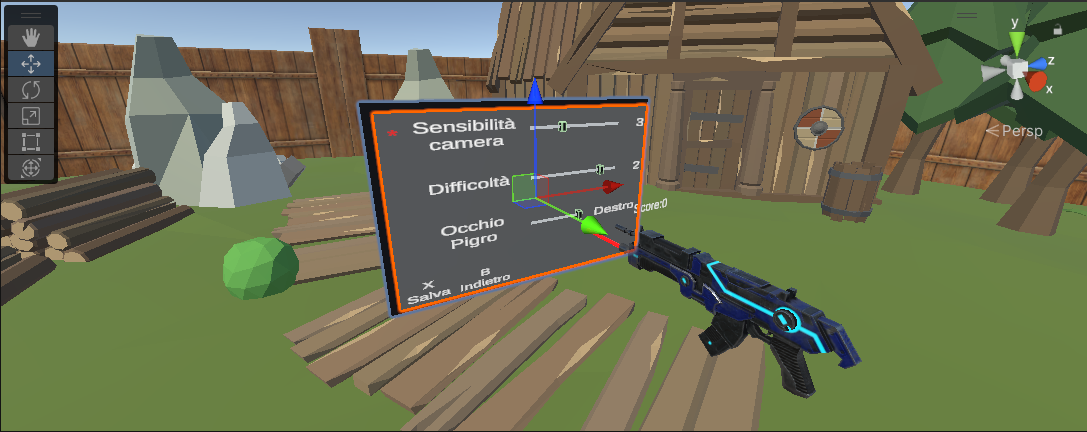
\includegraphics[width=0.8\linewidth]{image/menu_scena}
    	\caption{Vista del menu nella finestra \textit{Scene}}
    	\label{fig:menu_scena}
    \end{figure}
    In questo modo l'effetto ottenuto\ref{fig:menu_simulator} rispetta il principio citato prima.
     \begin{figure}[H]
    	\centering
    	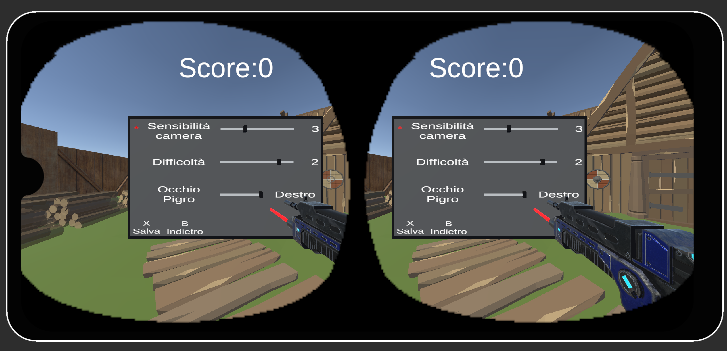
\includegraphics[width=0.8\linewidth]{image/menu_simulatore}
    	\caption{Vista del menu nella finestra \textit{simulator}}
    	\label{fig:menu_simulator}
    \end{figure}
    Dopo aver progettato e creato i componenti sopra citati, mi sono cimentato nella creazione dei vari livelli durante la \textbf{fase di sviluppo}. Il punto focale era quello di ricreare un ambiente in grado di stimolare sia l'occhio pigro che la curiosità dei pazienti. Ho cercato di rendere i singoli livelli intrattenenti, per mantenere l'interesse del giocatore.
    \subsubsection{Fase di sviluppo}
    Dopo aver completato la fase di progettazione e creazione dei vari componenti del gioco, mi sono concentrato sulla fase di sviluppo vera e propria. Durante questa fase, ho lavorato alla creazione dei singoli livelli del gioco, con l'obiettivo di rendere l'esperienza di gioco il più coinvolgente possibile. In questa sezione, descriverò il processo di sviluppo dei vari livelli.
    Per prima cosa sono andato ad importare gli Asset, di costruzioni, oggetti, ecc, in modo da potermi focalizzare su altri aspetti che ho reputato importanti.
    Gli asset che ho utilizzato sono:
    \begin{itemize}
    	\item Rocce\cite{Rock_asset}
    	\item Asset medievale\cite{Pack_asset}, contenente edifici, alberi e oggetti medievali. 
    	\item Muri\cite{Wall_asset}, contente i vari muri che circondano ogni livello.
    	\item Curva di Bézier\cite{Pack_asset}, il quale mi ha permesso di ricreare i target in movimento.
    \end{itemize}
    Dopo aver selezionato i singoli asset, sono andato ad assemblare il personaggio giocante, formato principalmente dagli script:
    \begin{itemize}
        \item Camera, in cui vado a ruotare e/o muovere l'oggetto \textit{testa}, contenente le due telecamere.
        \item GestioneTwo, dove mi sono concentrato sulla gestione delle due telecamere del gioco, ricreando l'effetto trasparenza e di profondità.
        \item Move, è uno script che ho sviluppato per gestire il movimento all'interno del gioco,questo script è stata fondamentale per garantire un'esperienza di gioco coinvolgente e immersiva.
        \item Shoot, riguarda l'implementazione di un azione fondamentale del gioco, il quale permette hai giocatori di raccogliere punti sparando a target disseminati nella mappa
        \item Teleporter, è uno script che ho creato per gestire il teletrasporto all'interno del gioco. Questo elemento è stato implementato per garantire una seconda opzione di movimento nel caso in cui il motion sickness\cite{mottion_sickness} dovesse influenzare negativamente l'esperienza di gioco degli utenti.
    \end{itemize}
    Gli script sopra citati, vengo organizzati seguendo uno scema gerarchico, fig:\ref{fig:script_character}, essi compongono il personaggio effettivo, il componente più importate del gioco
    \begin{figure}[H]
    	\centering
    	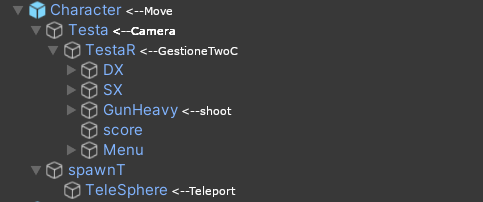
\includegraphics[width=0.8\linewidth]{image/script_character}
    	\caption{Organizzazione script}
    	\label{fig:script_character}
    \end{figure}
    Oltre agli elementi sopra citati sono contenuti al interno altri elementi, tra cui:
    \begin{itemize}
        \item DX e SX, non sono altro che le due telecamere.
        \item score, il quale visualizza il punteggio.
        \item Menu, implementa il sistema menu, descritto nel paragrafo precedente.
        \item spawnT, consente di impostare la posizione di origine dell'oggetto chiamato \textit{TeleSphere}, il quale può essere spostato in modo che funga da punto di riferimento per il teletrasporto.
    \end{itemize}
    Dopo aver costruito il personaggio giocante, sono andato a creare il terreno di gioco, disseminandolo con rocce\cite{Rock_asset}, edifici ed oggetti\cite{Pack_asset} di scena.
    Uno degli aspetti fondamentali è stato il posizionamento e la scelta degli oggetti "OcchioMalato", in quanto l'obiettivo principale è quello di andare a stimolare efficacemente l'occhio pigro, costringendo il paziente a prestare attenzione agli elementi del paesaggio.
    Legato a questo, ho disseminato ogni livello con un determinato numero di target fissi e/o in movimento, i quali sono essenziali per il proseguo del gioco e della terapia.
    Per quanto riguarda i target sono composti da un singolo script, nel cosa di quelli statici, invece per quelli in movimento abbiamo anche lo script per le curve di Bézier\cite{Pack_asset}.
    \textbf{Le curve di Bézier}\cite{Path_asset}, sono utilizzate principalmente in ambito grafico e di progettazione assistita dal computer (CAD), in questo caso sono state usate per delineare il percorso che i target devono seguire. Queste curve sono particolarmente utili per creare forme e traiettorie fluide e precise utilizzando un insieme di punti di controllo.
    Le curve sono state rappresentate in verde nella figura\ref{fig:mappa}.
     \begin{figure}[H]
    	\centering
    	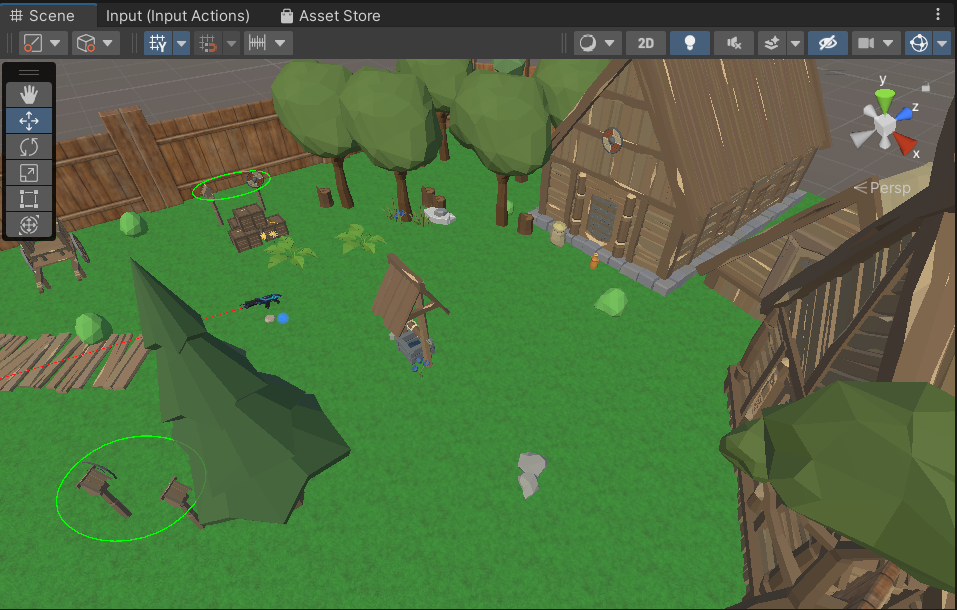
\includegraphics[width=0.8\linewidth]{image/mappa}
    	\caption{Secondo livello}
    	\label{fig:mappa}
    \end{figure}
    \subsection{Problemi}
    In questo paragrafo elencherò le limitazioni e le forzature che ho introdotto nel progetto per garantirne la stabilità. Come già accennato in precedenza\ref{chap:cardboard_motivi}, l'utilizzo del Cardboard mi ha fornito un set di tecnologie molto utili, ma ha anche comportato una limitazione tecnica significativa. Lo smartphone utilizzato con il Cardboard non è in grado di elaborare immagini troppo complesse, il che mi ha costretto a scegliere uno stile low poly per gli asset  gioco.
      \begin{figure}[H]//inserire foto immagini low poly albero
    	\centering
    	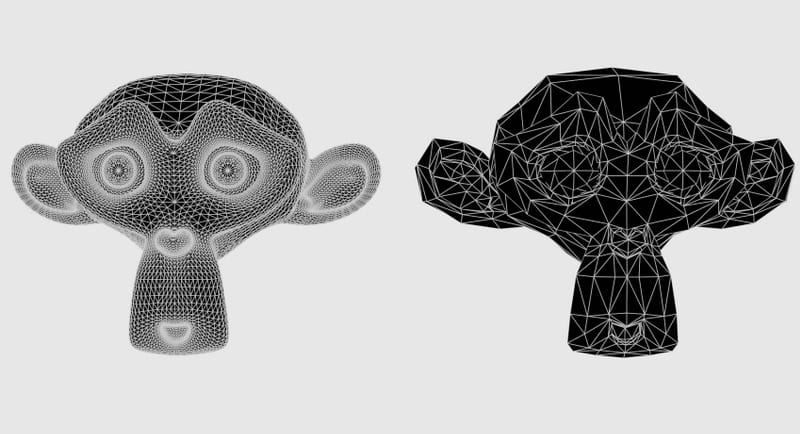
\includegraphics[width=0.8\linewidth]{image/low_hight}
    	\caption{Differenza High Poly e Low Poly  }
    	\label{fig:low_hight}
    \end{figure}
    Questa limitazione si può anche osservare dagli alberi scelti i quali non presentano foglie ma chiome stilizzate.
    Collegato a questo andrò a parlare della trasparenza, ampiamente discussa nei paragrafi precedenti, essa funziona andando a duplicare i vari oggetti, designati come "OcchioMalato", andando a cambiandone il materiale.
    L'operazione sopra descritta implica che lo smartphone dovrà renderizzare e tenere in memoria nel peggior dei casi, il doppio degli elementi, questo implica che bisogna scegliere saggiamente a quali oggetti impostare il tag "OcchioMalato".
    \subsection{Sviluppi futuri}
    
    \newpage
    \null
    \newpage
  
    
	\bibliographystyle{unsrt}
	\bibliography{./reference/r_web.bib}
	
	\thanks{Cristina D'avena,Matteo Verzeroli,Luca }

\end{document}